\begin{abstract}
This document contains a problem based on properties of triangle.
\end{abstract}

Download the python codes from 
%
\begin{lstlisting}
https://github.com/pranaya14014/EE5609/tree/master/Assignment3/code
\end{lstlisting}
%
and latex-tikz codes from 
%
\begin{lstlisting}
https://github.com/pranaya14014/EE5609/tree/master/Assignment3
\end{lstlisting}
%
\section{PROBLEM}
ABC is a right angled triangle in which $\angle A=90\degree$ and AB=AC find $\angle B$ and $\angle C$. 

\section{SOLUTION}
\textbf{Given:} Consider a right $\triangle{ABC}$ with sides AB, BC, AC right angled at $\angle A$ and AB=AC.\\

\textbf{Property used:} Angle opposite to equal sides are equal that is $\angle ABC = \angle ACB $\\

Using property that sum of all the angles of the triangle is equal to $180 \degree$.

\begin{align}
    \angle BAC + \angle ABC + \angle ACB = 180\degree
\end{align}

Let $\angle ABC = \angle ACB = x $

\begin{align}
    90\degree + x + x = 180 \degree
\\
    2x = 90\degree
\\
    x=45\degree
\end{align}

Hence $\angle B = \angle C = 45\degree$.

\begin{figure}[h!]
\begin{center}
	\resizebox{\columnwidth/1}{!}{

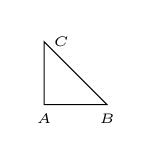
\begin{tikzpicture}[scale = 0.8, style={font=\tiny}]
\draw (0,0) node[anchor=north]{$A$}
  -- (0,1) node[anchor=west]{$C$}
  -- (1,0) node[anchor=north]{$B$}
  -- cycle;
\end{tikzpicture}}
\end{center}
\caption{Right Angled Triangle}
\label{fig:Triangle}
\end{figure}

